%
%===============>>  ГРУППА 9-2 МОДУЛЬ 8  <<=============
%
\setmodule{8}

%BEGIN_FOLD % ====>>_____ Занятие 1 _____<<====
\begin{class}[number=1]
	\begin{listofex}
		\item Переведите в десятичную дробь:
		\begin{tasks}(4)
			\task \( \dfrac{1}{4} \)
			\task \( \dfrac{2}{5} \)
			\task \( \dfrac{3}{8} \)
			\task \( \dfrac{8}{25} \)
			\task \( \dfrac{15}{10} \)
			\task \( \dfrac{1}{100} \)
			\task \( \dfrac{3}{200} \)
			\task \( \dfrac{7}{500} \)
		\end{tasks}
		\item Вычислите:
		\begin{tasks}(4)
			\task \( \dfrac{4}{25}+\dfrac{15}{4} \)
			\task \( \dfrac{9}{4}+\dfrac{8}{5} \)
			\task \( \dfrac{19}{2}-\dfrac{7}{25} \)
			\task \( \dfrac{3}{2}-\dfrac{9}{5} \)
			\task \( \dfrac{9}{5}\cdot\dfrac{2}{3} \)
			\task \( \dfrac{21}{5}\cdot\dfrac{3}{7} \)
			\task \( \dfrac{14}{5}:\dfrac{7}{2} \)
			\task \( \dfrac{3}{5}:\dfrac{4}{35} \)
		\end{tasks}
		\item Вычислите:
		\begin{tasks}(2)
			\task \( \left( \dfrac{19}{8}+\dfrac{11}{12} \right):\dfrac{5}{48} \)
			\task \( \left( \dfrac{14}{11}+\dfrac{17}{10} \right)\cdot\dfrac{11}{15} \)
			\task \( \left( \mfrac{2}{3}{4}+\mfrac{2}{1}{5} \right)\cdot16 \)
			\task \( \mfrac{1}{8}{17}:\left( \dfrac{12}{17}+\mfrac{2}{7}{11} \right) \)
		\end{tasks}
		\item Какое из данных ниже чисел принадлежит промежутку \( [3;4] \)?
		\begin{tasks}(4)
			\task \( \dfrac{45}{19} \)
			\task \( \dfrac{52}{19} \)
			\task \( \dfrac{68}{19} \)
			\task \( \dfrac{77}{19} \)
		\end{tasks}
		\item Какому из данных промежутков принадлежит число \( \dfrac{5}{9} \)?
		\begin{tasks}(4)
			\task \( [0,5; \, 0,6] \)
			\task \( [0,6 \, 0,7] \)
			\task \( [0,7 \, 0,8] \)
			\task \( [0,8 \, 0,9] \)
		\end{tasks}
		\item Вычислите:
		\begin{tasks}(4)
			\task \( \dfrac{1}{4}+0,7 \)
			\task \( \dfrac{1}{2}+0,07 \)
			\task \( \dfrac{24}{3,2\cdot2} \)
			\task \( \dfrac{27}{3\cdot4,5} \)
			\task \( \dfrac{11}{4,4\cdot2,5} \)
			\task \( \dfrac{7}{12,5\cdot1,4} \)
			\task \( \dfrac{0,9}{1+\frac{1}{8}} \)
			\task \( \dfrac{0,3}{1+\frac{1}{9}} \)
		\end{tasks}
	\end{listofex}
\end{class}
%END_FOLD

%BEGIN_FOLD % ====>>_____ Занятие 2 _____<<====
\begin{class}[number=2]
	\begin{listofex}
		\item Вычислите:
		\begin{tasks}(3)
			\task \( \dfrac{6,9-1,5}{2,4} \)
			\task \( \dfrac{2,4}{2,9-1,4} \)
			\task \( \dfrac{9,4}{4,1+5,3} \)
			\task \( \dfrac{6,9+4,1}{0,2} \)
			\task \( \dfrac{4,8\cdot0,4}{0,6} \)
			\task \( \dfrac{21}{0,3\cdot2,8} \)
			\task \( 0,6\cdot(-10)^3+50 \)
			\task \( -0,2\cdot(-10)^2+55 \)
			\task \( 30-0,8\cdot(-10)^2 \)
			\task \( 5,4\cdot0,8+0,08 \)
			\task \( 0,03\cdot0,3\cdot30000 \)
			\task \( 0,007\cdot7\cdot700 \)
		\end{tasks}
		\item Какому из промежутков принадлежит число \( \dfrac{7}{11} \)?
		\begin{tasks}(4)
			\task \( [0,4; \, 0,5] \)
			\task \( [0,5; \, 0,6] \)
			\task \( [0,6; \, 0,7] \)
			\task \( [0,7; \, 0,8] \)
		\end{tasks}
		\item Известно, что \( 0<a<1 \). Выберите наименьшее число
		\begin{tasks}(4)
			\task \( a^2 \)
			\task \( a^3 \)
			\task \( -a \)
			\task \( \dfrac{1}{a} \)
		\end{tasks}
		\item Известно, что \( a<b<0 \). Выберите наименьшее из чисел.
		\begin{tasks}(4)
			\task \( a-1 \)
			\task \( b-1 \)
			\task \( ab \)
			\task \( -b \)
		\end{tasks}
		\item Известно, что \( a \) и \( b \) --- положительные числа и \( a>b \). Сравните \( \dfrac{1}{a} \) и \( \dfrac{1}{b} \).
		\begin{tasks}(4)
			\task \( \dfrac{1}{a}>\dfrac{1}{b} \)
			\task \( \dfrac{1}{a}<\dfrac{1}{b} \)
			\task \( \dfrac{1}{a}=\dfrac{1}{b} \)
			\task Сравнить невозможно
		\end{tasks}
		\item Известно, что \( a>b>c \). Какое из следующих чисел отрицательно?
		\begin{tasks}(4)
			\task \( a-b \)
			\task \( a-c \)
			\task \( b-c \)
			\task \( c-b \)
		\end{tasks}
		\item Какое из следующих чисел заключено между числами \( \dfrac{1}{6} \) и \( \dfrac{1}{4} \)?
		\begin{tasks}(4)
			\task \( 0,1 \)
			\task \( 0,2 \)
			\task \( 0,3 \)
			\task \( 0,4 \)
		\end{tasks}
		\item Какое из приведенных ниже неравенств является верным при любых значениях \( a \) и \( b \), удовлетворяющих условию \( a>b \)?
		\begin{tasks}(4)
			\task \( b-a<-2 \)
			\task \( a-b>-1 \)
			\task \( a-b<3 \)
			\task \( b-a>-3 \)
		\end{tasks}
	\newpage
		\item Значение какого из данных выражений положительно, если известно, что \( x>0 \), \( y<0 \)?
		\begin{tasks}(4)
			\task \( xy \)
			\task \( (x-y)y \)
			\task \( (y-x)y \)
			\task \( (y-x)x \)
		\end{tasks}
		\item Вычислите:
		\begin{tasks}(2)
			\task \( \left( \dfrac{17}{8}-\dfrac{11}{20} \right):\dfrac{5}{46} \)
			\task \( \mfrac{4}{3}{4}:\left( \mfrac{1}{1}{15}+\dfrac{3}{5} \right) \)
			\task \( \mfrac{1}{1}{12}:\left( \mfrac{1}{13}{18}-\mfrac{2}{5}{9} \right) \)
			\task \( \left( \mfrac{1}{11}{16}-\mfrac{3}{7}{8} \right)\cdot4 \)
			\task \( \left( \dfrac{5}{6}+\mfrac{1}{1}{10} \right)\cdot24 \)
			\task \( \dfrac{1}{\frac{1}{22}+\frac{1}{18}} \)
			\task \( \dfrac{1}{\frac{1}{36}-\frac{1}{44}} \)
			\task \( \dfrac{1}{\frac{1}{33}+\frac{1}{12}} \)
		\end{tasks}
	\end{listofex}
\end{class}
%END_FOLD

%BEGIN_FOLD % ====>>_ Домашняя работа 1 _<<====
\begin{homework}[number=1]
	\begin{listofex}
		\item Вычислите:
		\begin{tasks}(3)
			\task \( \left( \dfrac{10}{13}+\dfrac{15}{4} \right)\cdot\dfrac{26}{5} \)
			\task \( \mfrac{2}{2}{5}:\left( \dfrac{9}{10}-\mfrac{1}{5}{14} \right) \)
			\task \( \dfrac{1}{\frac{1}{72}-\frac{1}{99}} \)
			\task \( \dfrac{11}{4,4\cdot2,5} \)
			\task \( \dfrac{2,7}{1,7+0,1} \)
			\task \( \dfrac{0,3\cdot4,4}{0,8} \)
		\end{tasks}
		\item Вычислите:
		\begin{tasks}(2)
			\task \( -2,54+6,6\cdot4,1 \)
			\task \( 80+0,9\cdot(-10)^3 \)
			\task \( 0,7\cdot(-10)^3-20 \)
			\task \( 45+0,6\cdot(-10)^2 \)
			\task \( -0,7\cdot(-10)^2+90 \)
			\task \( 400\cdot0,004\cdot40 \)
		\end{tasks}
		\item О числах \( a \), \( b \), \( c \) и \( d \) известно, что \( a>b \), \( b<c \), \( d=c \). Сравните числа \( d \) и \( a \).
		\begin{tasks}(4)
			\task \( d=a \)
			\task \( d>a \)
			\task \( d<a \)
			\task Сравнить невозможно
		\end{tasks}
		\item Какому из данных промежутков принадлежит число \( \dfrac{5}{11} \)?
		\begin{tasks}(1)
			\task \( [0,2; \, 0,3] \)
			\task \( [0,3; \, 0,4] \)
			\task \( [0,4; \, 0,5] \)
			\task \( [0,5; \, 0,6] \)
		\end{tasks}
		\item Какое из чисел принадлежит отрезку \( [8; \, 9] \)?
		\begin{tasks}(4)
			\task \( \dfrac{46}{7} \)
			\task \( \dfrac{53}{7} \)
			\task \( \dfrac{55}{7} \)
			\task \( \dfrac{61}{7} \)
		\end{tasks}
	\end{listofex}
\end{homework}
%END_FOLD

%BEGIN_FOLD % ====>>_____ Занятие 3 _____<<====
\begin{class}[number=3]
	\begin{listofex}
		\item Переведите в десятичную дробь:
		\begin{tasks}(4)
			\task \( \dfrac{5}{10} \)
			\task \( \dfrac{41}{100} \)
			\task \( \dfrac{89}{1000} \)
			\task \( \dfrac{555}{100} \)
			\task \( \dfrac{1}{20} \)
			\task \( \dfrac{3}{25} \)
			\task \( \dfrac{9}{8} \)
			\task \( \dfrac{6}{125} \)
		\end{tasks}
		\item Выполните умножение:
		\begin{tasks}(4)
			\task \( 0,6\cdot0,48 \)
			\task \( 1,5\cdot8,99 \)
			\task \( 9,3\cdot7,1 \)
			\task \( 7,01\cdot150,02 \)
			\task \( 100,23\cdot8,96 \)
			\task \( 6,12\cdot7,36 \)
			\task \( 2,39\cdot7,12 \)
			\task \( 19,03\cdot0,002 \)
		\end{tasks}
		\item Вычислите:
		\begin{tasks}(4)
			\task \( \dfrac{9,4}{4,1+5,3} \)
			\task \( \dfrac{5,6}{1,9-7,5} \)
			\task \( \dfrac{7,5+3,5}{2,5} \)
			\task \( \dfrac{9,5+8,9}{2,3} \)
			\task \( \dfrac{2,7}{1,4+0,1} \)
			\task \( \dfrac{1,8+1,9}{3,7} \)
			\task \( \dfrac{4,7-1,4}{7,5} \)
			\task \( \dfrac{2,6-2,6}{7,8} \)
		\end{tasks}
		\item Какому из промежутков принадлежит число \( \dfrac{7}{11} \)?
		\begin{tasks}(4)
			\task \( [0,4; \, 0,5] \)
			\task \( [0,5; \, 0,6] \)
			\task \( [0,6; \, 0,7] \)
			\task \( [0,7; \, 0,8] \)
		\end{tasks}
		\item Известно, что \( 0<a<1 \). Выберите наименьшее число
		\begin{tasks}(4)
			\task \( a^2 \)
			\task \( a^3 \)
			\task \( -a \)
			\task \( \dfrac{1}{a} \)
		\end{tasks}
		\item Известно, что \( a<b<0 \). Выберите наименьшее из чисел.
		\begin{tasks}(4)
			\task \( a-1 \)
			\task \( b-1 \)
			\task \( ab \)
			\task \( -b \)
		\end{tasks}
		\item Известно, что \( a \) и \( b \) --- положительные числа и \( a>b \). Сравните \( \dfrac{1}{a} \) и \( \dfrac{1}{b} \).
		\begin{tasks}(4)
			\task \( \dfrac{1}{a}>\dfrac{1}{b} \)
			\task \( \dfrac{1}{a}<\dfrac{1}{b} \)
			\task \( \dfrac{1}{a}=\dfrac{1}{b} \)
			\task Сравнить невозможно
		\end{tasks}
		\item Известно, что \( a>b>c \). Какое из следующих чисел отрицательно?
		\begin{tasks}(4)
			\task \( a-b \)
			\task \( a-c \)
			\task \( b-c \)
			\task \( c-b \)
		\end{tasks}
		\item Какое из следующих чисел заключено между числами \( \dfrac{1}{6} \) и \( \dfrac{1}{4} \)?
		\begin{tasks}(4)
			\task \( 0,1 \)
			\task \( 0,2 \)
			\task \( 0,3 \)
			\task \( 0,4 \)
		\end{tasks}
		\item Какое из приведенных ниже неравенств является верным при любых значениях \( a \) и \( b \), удовлетворяющих условию \( a>b \)?
		\begin{tasks}(4)
			\task \( b-a<-2 \)
			\task \( a-b>-1 \)
			\task \( a-b<3 \)
			\task \( b-a>-3 \)
		\end{tasks}
		\newpage
		\item Значение какого из данных выражений положительно, если известно, что \( x>0 \), \( y<0 \)?
		\begin{tasks}(4)
			\task \( xy \)
			\task \( (x-y)y \)
			\task \( (y-x)y \)
			\task \( (y-x)x \)
		\end{tasks}
	\end{listofex}
\end{class}
%END_FOLD

%BEGIN_FOLD % ====>>_____ Занятие 4 _____<<====
\begin{class}[number=4]
	\begin{listofex}
		\item Занятие 4
	\end{listofex}
\end{class}
%END_FOLD

%BEGIN_FOLD % ====>>_ Домашняя работа 2 _<<====
\begin{homework}[number=2]
	\begin{listofex}
		\item Вычислите:
		\begin{tasks}(3)
			\task \( 5,6\cdot5,5-4,15 \)
			\task \( 5,3-9\cdot(-4,4) \)
			\task \( \dfrac{0,9+0,7}{3,2} \)
			\task \( \dfrac{9,4}{4,1+5,3} \)
			\task \( \dfrac{1,7+3,8}{2,2} \)
			\task \( \dfrac{7,2-6,1}{2,2} \)
			\task \( \dfrac{3,7\cdot7,5}{7,4} \)
			\task \( \dfrac{5,6\cdot0,3}{0,8} \)
		\end{tasks}
		\item О числах \( a \), \( b \), \( c \) и \( d \) известно, что \( a<b \), \( b<c \), \( d>c \). Сравнитe числа \( d \) и \( a \).
		\begin{tasks}(4)
			\task \( d=a \)
			\task \( d>a \)
			\task \( d<a \)
			\task Сравнить невозможно
		\end{tasks}
		\item Известно, что \( a<b<0 \). Выберите наименьшее из чисел.
		\begin{tasks}(4)
			\task \( a-1 \)
			\task \( b-1 \)
			\task \( ab \)
			\task \( -b \)
		\end{tasks}
		\item Известно, что \( a \) и \( b \) --- положительные числа и \( a>b \). Сравните \( \dfrac{1}{a} \) и \( \dfrac{1}{b} \).
		\begin{tasks}(4)
			\task \( \dfrac{1}{a}>\dfrac{1}{b} \)
			\task \( \dfrac{1}{a}<\dfrac{1}{b} \)
			\task \( \dfrac{1}{a}=\dfrac{1}{b} \)
			\task Сравнить невозможно
		\end{tasks} 
	\end{listofex}
\end{homework}
%END_FOLD

%BEGIN_FOLD % ====>>_____ Занятие 5 _____<<====
\begin{class}[number=5]
	\begin{listofex}
		\item Вычислите:
		\begin{tasks}(2)
			\task \( \left( \dfrac{17}{8}-\dfrac{11}{20} \right):\dfrac{5}{46} \)
			\task \( \mfrac{4}{3}{4}:\left( \mfrac{1}{1}{15}+\dfrac{3}{5} \right) \)
			\task \( \mfrac{1}{1}{12}:\left( \mfrac{1}{13}{18}-\mfrac{2}{5}{9} \right) \)
			\task \( \left( \mfrac{1}{11}{16}-\mfrac{3}{7}{8} \right)\cdot4 \)
			\task \( \left( \dfrac{5}{6}+\mfrac{1}{1}{10} \right)\cdot24 \)
			\task \( \dfrac{1}{\frac{1}{22}+\frac{1}{18}} \)
			\task \( \dfrac{1}{\frac{1}{36}-\frac{1}{44}} \)
			\task \( \dfrac{1}{\frac{1}{33}+\frac{1}{12}} \)
		\end{tasks}
		\item На координатной прямой отмечено число \( c \). Расположите в порядке убывания числа \( c \), \( c^2 \) и \( \dfrac{1}{c} \). 
		\begin{center}
			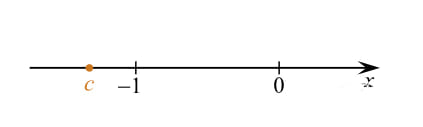
\includegraphics[align=t, width=0.5\linewidth]{\picpath/G93M8L5}
		\end{center}
	\begin{tasks}(2)
		\task \( c^2; \, c; \, \dfrac{1}{c} \)
		\task \( c^2; \, \dfrac{1}{c}; \, c \)
		\task \( c; \, c^2; \, \dfrac{1}{c} \)
		\task \( c; \, \dfrac{1}{c}; \, c^2;  \)
	\end{tasks}
		\item На координатной прямой отмечены числа \( a \) и \( x \).
		\begin{center}
			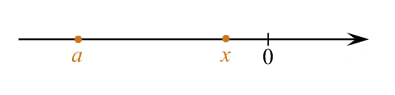
\includegraphics[align=t, width=0.5\linewidth]{\picpath/G93M8L5-1}
		\end{center}
		Какое из следующих чисел наименьшее?
		\begin{tasks}(4)
			\task \( a+x \)
			\task \( \dfrac{x}{2} \)
			\task \( -a \)
			\task \( a-x \)
		\end{tasks}
		\item На координатной прямой отмечено число \( a \).
		\begin{center}
			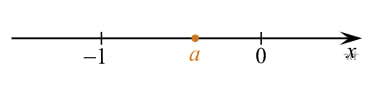
\includegraphics[align=t, width=0.5\linewidth]{\picpath/G93M8L5-2}
		\end{center}
		Расположите в порядке возрастания числа \( a-1 \), \( \dfrac{1}{a} \), \( a \). 
		\begin{tasks}(2)
			\task \( a; \, \dfrac{1}{a}; \, a-1 \)
			\task \( a; \, a-1; \, \dfrac{1}{a} \)
			\task \( a-1; \, a; \, \dfrac{1}{a} \)
			\task \( \dfrac{1}{a}; \, a-1; \, a\)
		\end{tasks}
		\item На координатной прямой отмечено число \( a \).
		\begin{center}
			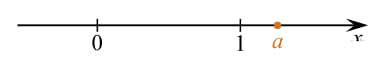
\includegraphics[align=t, width=0.5\linewidth]{\picpath/G93M8L5-3}
		\end{center}
		Найдите наибольшее из чисел \( a^2 \), \( a^3 \), \( a^4 \).
		\begin{tasks}(4)
			\task \( a^2 \)
			\task \( a^3 \)
			\task \( a^4 \)
			\task Не хватает данных для ответа
		\end{tasks}
		\item На координатной прямой точками отмечены числа \( \dfrac{6}{13} \); \( \dfrac{8}{17} \); \( 0,42 \); \( 0,45 \).
		\begin{center}
			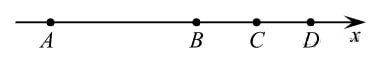
\includegraphics[align=t, width=0.5\linewidth]{\picpath/G93M8L5-4}
		\end{center}
		Какому числу соответствует точка \( B \)?
		\begin{tasks}(4)
			\task \( \dfrac{6}{13} \)
			\task \( \dfrac{8}{17} \)
			\task \( 0,42 \)
			\task \( 0,45 \)
		\end{tasks}
		\item Вычислите:
		\begin{tasks}(4)
			\task \( \dfrac{0,9+0,7}{3,2} \)
			\task \( \dfrac{4,7-1,4}{7,5} \)
			\task \( \dfrac{0,9+0,7}{3,2} \)
			\task \( \dfrac{6,3+4,3}{5,3} \)
			\task \( \dfrac{7,9+3,4}{0,2} \)
			\task \( \dfrac{1,3+9,2}{1,5} \)
			\task \( \dfrac{0,9+0,7}{3,2} \)
			\task \( \dfrac{0,5-1,5}{0,8} \)
			\task \( \dfrac{24}{4\cdot4,8} \)
			\task \( \dfrac{9}{4,5\cdot2,5} \)
			\task \( \dfrac{22}{4,4\cdot2,5} \)
			\task \( \dfrac{4,4\cdot7,2}{0,9} \)
		\end{tasks}
	\end{listofex}
\end{class}
%END_FOLD

%BEGIN_FOLD % ====>>_____ Занятие 6 _____<<====
\begin{class}[number=6]
	\begin{listofex}
		\item Одна из точек, отмеченных на координатной прямой, соответствует числу \( \dfrac{3}{8} \).  Какая это точка?
		\begin{center}
			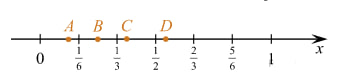
\includegraphics[align=t, width=0.5\linewidth]{\picpath/G93M8L6}
		\end{center}
		\begin{tasks}(4)
			\task \( A \)
			\task \( B \)
			\task \( C \)
			\task \( D \)
		\end{tasks}
		\item Одно из чисел \( \dfrac{5}{6} \); \( \dfrac{5}{7} \); \( \dfrac{5}{9} \); \( \dfrac{5}{12} \) отмечено на координатной прямой точкой \( A \). Укажите это число.
		\begin{center}
			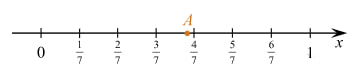
\includegraphics[align=t, width=0.5\linewidth]{\picpath/G93M8L6-1}
		\end{center}
		\begin{tasks}(4)
			\task \( \dfrac{5}{6} \)
			\task \( \dfrac{5}{7} \)
			\task \( \dfrac{5}{9} \)
			\task \( \dfrac{5}{12} \)
		\end{tasks}
		\item Какому из следующих чисел соответствует точка, отмеченная на координатной прямой?
		\begin{center}
			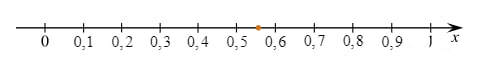
\includegraphics[align=t, width=0.5\linewidth]{\picpath/G93M8L6-2}
		\end{center}
		\begin{tasks}(4)
			\task \( \dfrac{10}{23} \)
			\task \( \dfrac{12}{23} \)
			\task \( \dfrac{13}{23} \)
			\task \( \dfrac{14}{23} \)
		\end{tasks}
		\item На координатной прямой точками \( A \), \( B \), \( C \) и \( D \) отмечены числа \( 0,098 \); \( -0,02 \); \( 0,09 \); \( 0,11 \). Какой точкой изображается число \( 0,09 \)?
		\begin{center}
			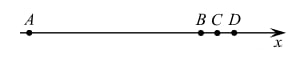
\includegraphics[align=t, width=0.5\linewidth]{\picpath/G93M8L6-3}
		\end{center}
		\begin{tasks}(4)
			\task \( A \)
			\task \( B \)
			\task \( C \)
			\task \( D \)
		\end{tasks}
		\item На координатной прямой отмечено число \( a \).
		\begin{center}
			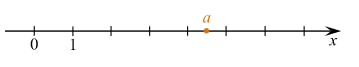
\includegraphics[align=t, width=0.5\linewidth]{\picpath/G93M8L6-5}
		\end{center}
		Какое из утверждений относительно этого числа является верным?
		\begin{tasks}(4)
			\task \( a-8>0 \)
			\task \( 7-a<0 \)
			\task \( a-3>0 \)
			\task \( 2-a>0 \)
		\end{tasks}
		\item На координатной прямой отмечены числа \( a \) и \( b \). Какое из следующих утверждений неверно?
		\begin{center}
			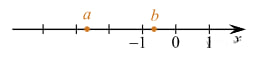
\includegraphics[align=t, width=0.5\linewidth]{\picpath/G93M8L6-6}
		\end{center}
		\begin{tasks}(2)
			\task \( a+b<0 \)
			\task \( -2<b-1<-1 \)
			\task \( a^2b<0 \)
			\task \( -a<0 \)
		\end{tasks}
		\item Решите уравнения:
		\begin{tasks}(2)
			\task\(4x+7=0\)
			\task \(2x+2=-3\)
			\task \(2-3(2x+2)=5-4x\)
			\task \(9-2(-4x+7)=7\)
			\task \(13+\dfrac{ x }{ 4 }=x+1\)
			\task \(\dfrac{ x-6 }{ 2 }-\dfrac{ x }{ 3 }=3\)
			\task \( \mfrac{5}{1}{2}x+\mfrac{3}{5}{6}=\mfrac{7}{3}{4}x+\mfrac{2}{2}{3} \)
			\task \( \mfrac{7}{1}{2}x+\mfrac{4}{1}{3}=\mfrac{3}{1}{9}+\mfrac{5}{5}{6}x \)
			\task \( \mfrac{10}{5}{14}-\left( x+\mfrac{2}{9}{34} \right)=\mfrac{4}{25}{34}  \)
			\task \( \mfrac{3}{8}{15}-\left( x+\mfrac{1}{2}{5} \right)=\dfrac{ 5 }{ 6 }  \)
		\end{tasks}
		\item Решите системы уравнений:
		\begin{itasks}[2]
			\task \exercise{191}
			\task \exercise{190}
			\task \exercise{206}
			\task \exercise{207}
		\end{itasks}
	\end{listofex}
\end{class}
%END_FOLD

%BEGIN_FOLD % ====>>_ Домашняя работа 3 _<<====
\begin{homework}[number=3]
	\begin{listofex}
		\item Известно, что число \( m \) отрицательное. На каком из рисунков точки с координатами \( 0 \), \( m \), \( 2m \), \( m^2 \) расположены на координатной прямой в правильном порядке?
		\begin{center}
			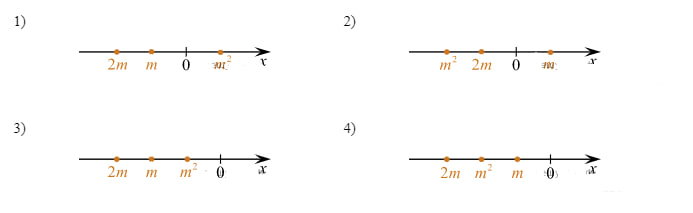
\includegraphics[align=t, width=1\linewidth]{\picpath/G93M8L6-4}
		\end{center}
		\begin{tasks}(4)
			\task \( 1 \)
			\task \( 2 \)
			\task \( 3 \)
			\task \( 4 \)
		\end{tasks}
		\item Одно из чисел \( \dfrac{81}{17} \), \( \dfrac{90}{17} \), \( \dfrac{99}{17} \), \( \dfrac{108}{17} \) отмечено на прямой точкой. Укажите это число.
		\begin{center}
			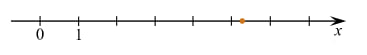
\includegraphics[align=t, width=0.9\linewidth]{\picpath/G93M8H3}
		\end{center}
		\begin{tasks}(4)
			\task \( \dfrac{81}{17} \)
			\task \( \dfrac{90}{17} \)
			\task \( 3 \)\( \dfrac{99}{17} \)
			\task \(\dfrac{108}{17}\)
		\end{tasks}
		\item Вычислите:
		\begin{tasks}(2)
			\task \( 30-0,8\cdot(-10)^2 \)
			\task \( -0,7\cdot(-10)^2+90 \)
			\task \( 2,5\cdot3,5-0,35 \)
			\task \( 6,8-11\cdot(-6,1) \)
			\task \( 0,09\cdot0,9\cdot9000 \)
			\task \( 0,02\cdot0,00002\cdot0,000002\)
		\end{tasks}
		\item Решите уравнения:
		\begin{tasks}(2)
			\task \( -10x+2=0 \)
			\task \( x-2=-3x \)
			\task \( 4(x+10)=-1 \)
			\task \( -9(8-9x)=4x+5 \)
			\task \( 9-2(-4x+7)=7 \)
			\task \( \dfrac{x}{12}+\dfrac{x}{8}+x=-\dfrac{29}{6} \)
		\end{tasks}
		\item Решите систему уравнений: \(\begin{cases}  3x+2y=8  \\  4x-y=7 \end{cases}\). В ответ запишите \( x+y \).
	\end{listofex}
\end{homework}
%END_FOLD

%BEGIN_FOLD % ====>>_____ Занятие 7 _____<<====
\begin{class}[number=7]
	\begin{listofex}
		\item Решите уравнения:
		\begin{tasks}(2)
			\task \( -2(-4+7x)+8x=3 \)
			\task \( 1-7(4+2x)=-9-4x \)
			\task \( 9+2(3-4x)=3x-3 \)
			\task \( -6x-4(9-7x)=-5x+1 \)
		\end{tasks}
		\item Решите уравнения:
		\begin{tasks}(2)
			\task \( 3-\dfrac{x}{3}=\dfrac{x}{2} \)
			\task \( 3-\dfrac{x}{7}=\dfrac{x}{3} \)
			\task \( \dfrac{6x+8}{2}+5=\dfrac{5x}{3} \)
			\task \( \dfrac{9x+6}{7}+3=\dfrac{7x}{6} \)
			\task \( \dfrac{4x+7}{3}+2=\dfrac{7x}{2} \)
			\task \( \dfrac{3x-2}{4}-\dfrac{x}{3}=2 \)
		\end{tasks}
		\item Найдите значение выражений:
		\begin{tasks}(4)
			\task \( \dfrac{3^7}{81} \)
			\task \( \dfrac{27^5}{9^6} \)
			\task \( \dfrac{81^5}{27^6} \)
			\task \( \dfrac{125^6}{25^8} \)
			\task \( \dfrac{10^6}{2^5\cdot5^4} \)
			\task \( \dfrac{24^4}{3^2\cdot8^3} \)
			\task \( \dfrac{(3\cdot10)^8}{3^6\cdot10^7} \)
			\task \( \dfrac{(2\cdot3)^5}{2^4\cdot3^3} \)
		\end{tasks}
		\item Найдите значение выражений:
		\begin{tasks}(3)
			\task \( 4^{-10}\cdot(4^3)^4 \)
			\task \( 5^{-7}\cdot(5^5)^2 \)
			\task \( 3^{-11}\cdot(3^5)^2 \)
			\task \( 7^4\cdot(7^2)^{-3} \)
			\task \( 5^6\cdot(5^{-4})^2 \)
			\task \( 9^{-5}\cdot(9^3)^2 \)
		\end{tasks}
		\item Чему равно значение выражений?
		\begin{tasks}(3)
			\task \( (3\sqrt{2})^2 \)
			\task \( (5\sqrt{3})^2 \)
			\task \( (2\sqrt{7})^2 \)
		\end{tasks}
		\item Найдите значение выражения \( \dfrac{a^{23}\cdot(b^5)^4}{(a\cdot b)^{20}} \) при \( a=2 \) и \( b=\sqrt{2} \).
		\item Найдите значение выражения \( \dfrac{a^{17}\cdot(b^5)^3}{(a\cdot b)^{15}} \) при \( a=7 \) и \( b=\sqrt{7} \).
		\item Найдите значение выражений:
		\begin{tasks}(3)
			\task \( 5\sqrt{11}\cdot2\sqrt{2}\cdot\sqrt{22} \)
			\task \( \sqrt{4\cdot12}\cdot\sqrt{21} \)
			\task \( \sqrt{2\cdot45}\cdot\sqrt{10} \)
			\task \( 3\sqrt{19}\cdot4\sqrt{2}\cdot\sqrt{38} \)
			\task \( 3\sqrt{11}\cdot4\sqrt{2}\cdot\sqrt{22} \)
			\task \( \sqrt{45}\cdot\sqrt{605} \)
		\end{tasks}
	\end{listofex}
\end{class}
%END_FOLD

=%BEGIN_FOLD % ====>>_ Проверочная работа _<<====
\begin{exam}
	\begin{listofex}
		\item Проверочная
	\end{listofex}
\end{exam}
%END_FOLD